%\documentclass[hyperref={pdfpagelabels=false},slidetop,9pt]{beamer}
\documentclass[slidetop,8pt]{beamer}
\usepackage[T1]{fontenc}
\usepackage[utf8]{inputenc}
\newcommand{\id}{54}
\newcommand{\nom}{Liaisons mécaniques}
\newcommand{\sequence}{04}
\newcommand{\num}{01}
\newcommand{\type}{TP}
\newcommand{\descrip}{Modélisation d'un solide. Comportement des liaisons mécaniques. Modéliser les mécanismes du laboratoire par un schéma cinématique, paramétré.}
\newcommand{\competences}{A3-C4: Analyse d'architecture et de comportement \\ &  Mod1-C1: Isolement d'un solide ou d'un système de solides \\ &  Mod2-C10-1: Modèle de solide indéformable \\ &  Mod2-C11: Modélisation géométrique et cinématique des mouvements entre solides indéformables \\ &  Mod2-C12: Modélisation cinématique des liaisons entre solides \\ &  Mod2-C15: Modélisation des actions mécaniques \\ &  Rés-C6: Utilisation d'un solveur ou d'un logiciel multi physique \\ &  Com1-C1: Différents descripteurs introduits dans le programme \\ &  Com2-C4: Outils de communication}
\newcommand{\nbcomp}{9}
\newcommand{\systemes}{Plateforme Stewart}
\newcommand{\systemessansaccent}{Plateforme Stewart}
\newcommand{\ilot}{2}
\newcommand{\ilotstr}{02}
\newcommand{\dossierilot}{\detokenize{Ilot_02 Plateforme Stewart}}
\newcommand{\imageun}{Plateforme}

\newcommand{\urlsysteme}{\href{https://www.costadoat.fr/systeme/57}{Ressources système}}
\newcommand{\matlabsimscape}{\href{https://github.com/Costadoat/Sciences-Ingenieur/raw/master/Systemes/Plateforme Stewart/Plateforme_Stewart_Simscape.zip}{Modèle Simscape}}
\newcommand{\solidworks}{\href{https://github.com/Costadoat/Sciences-Ingenieur/raw/master/Systemes/Plateforme Stewart/Plateforme_Stewart_Solidworks.zip}{Modèle Solidworks}}
\newcommand{\edrawings}{\href{https://github.com/Costadoat/Sciences-Ingenieur/raw/master/Systemes/Plateforme Stewart/Plateforme_Stewart.EASM}{Modèle eDrawings}}
\newcommand{\test}{Stewart_param1}
\newcommand{\testi}{Stewart_param2}
\newcommand{\testii}{Stewart_param3}
\newcommand{\testiii}{Stewart_param4}
\newcommand{\testiiii}{Stewart_euler}
\usepackage{etex}
\usepackage{tikz}
\usepackage[european]{circuitikz}
\usepackage{pgf}
\usepackage[all]{xy}
\usepackage{pgfpages}
\usepackage{graphbox}
\usepackage{pdfpages}
\usepackage[adobe-utopia]{mathdesign}
\usepackage{ifthen}
\usepackage{cancel}
\usepackage{framed}
\usepackage{subfig}
\usepackage{tabularx}
\usepackage{setspace}
\usepackage{soul}
\usepackage{schemabloc}
\usepackage{eqnarray}
\usepackage[dot, phantomtext]{dashundergaps}
\usepackage{media9}
\usepackage{multimedia}
\usepackage{textcomp}

\author{Renaud Costadoat}
\institute{Lycée Dorian}

\usepackage{multido}
\usepackage{multirow}
\usepackage{multicol} % Portions de texte en colonnes
\usepackage{flafter}%floatants après la référence

\usepackage{color}
\usepackage{xcolor}
\usepackage{colortbl}

\usepackage[gen]{eurosym}
\usepackage{tikz}
%\usepackage{pstricks,pst-node,pst-tree,pst-solides3d}
\usepackage{lmodern}
\usepackage[francais]{babel}
\usepackage{pslatex}
\usetheme{renaud}
\usepackage{times}
\usepackage{amsmath}
\usepackage{verbatim}
\usepackage{moreverb}
%\usetikzlibrary{arrows,shapes}
\usepackage{graphicx}
\usepackage{psfrag}
\usepackage{wrapfig}
\usepackage{etoolbox}

\definecolor{gris25}{gray}{0.75}
\definecolor{bleu}{RGB}{18,33,98}
\definecolor{bleuf}{RGB}{42,94,171}
\definecolor{bleuc}{RGB}{231,239,247}
\definecolor{rougef}{RGB}{185,18,27}
\definecolor{rougec}{RGB}{255,188,204}%255,230,231
\definecolor{vertf}{RGB}{103,126,82}
\definecolor{vertc}{RGB}{220,255,191}

\setlength\parindent{24pt}
\parskip 7.2pt
\parindent 8pt

\newenvironment{rem}[1][\hsize]%
{%
    \def\FrameCommand
   {%
\rotatebox{90}{\textit{\textsf{Remarque}}} 
       {\color{bleuf}\vrule width 3pt}%
       \hspace{0pt}%must no space.
       \fboxsep=\FrameSep\colorbox{bleuc}%
  }%
    \MakeFramed{\hsize#1\advance\hsize-\width\FrameRestore}%
}%
{\endMakeFramed}%


\newenvironment{savoir}[1][\hsize]%
{%
    \def\FrameCommand
    {%
\rotatebox{90}{\textit{\textsf{Savoir}}} 
        {\color{bleuf}\vrule width 3pt}%
        \hspace{0pt}%must no space.
        \fboxsep=\FrameSep\colorbox{bleuc}%
    }%
    \MakeFramed{\hsize#1\advance\hsize-\width\FrameRestore}%
}%
{\endMakeFramed}%

\newenvironment{prob}[1][\hsize]%
{%
    \def\FrameCommand%
    {%
\rotatebox{90}{\textit{\textsf{Problematique}}} 
        {\color{rougef}\vrule width 3pt}%
        \hspace{0pt}%must no space.
        \fboxsep=\FrameSep\colorbox{rougec}%
    }%
    \MakeFramed{\hsize#1\advance\hsize-\width\FrameRestore}%
}%
{\endMakeFramed}%

\newenvironment{obj}[1][\hsize]%
{%
    \def\FrameCommand%
    {%
\rotatebox{90}{\textit{\textsf{Objectif}}} 
        {\color{vertf}\vrule width 3pt}%
        \hspace{0pt}%must no space.
        \fboxsep=\FrameSep\colorbox{vertc}%
    }%
    \MakeFramed{\hsize#1\advance\hsize-\width\FrameRestore}%
}%
{\endMakeFramed}%

\newenvironment{defi}[1][\hsize]%
{%
    \def\FrameCommand%
    {%
\rotatebox{90}{\textit{\textsf{Definition}}} 
        {\color{bleuf}\vrule width 3pt}%
        \hspace{0pt}%must no space.
        \fboxsep=\FrameSep\colorbox{rougec}%
    }%
    \MakeFramed{\hsize#1\advance\hsize-\width\FrameRestore}%
}%
{\endMakeFramed}%


\newenvironment{hypo}[1][\hsize]%
{%
    \def\FrameCommand%
    {%
\rotatebox{90}{\textit{\textsf{Hypothèse\\}}} 
        {\color{bleuf}\vrule width 3pt}%
        \hspace{0pt}%must no space.
        \fboxsep=\FrameSep\colorbox{bleuc}%
    }%
    \MakeFramed{\hsize#1\advance\hsize-\width\FrameRestore}%
}%
{\endMakeFramed}%


\newenvironment{prop}[1][\hsize]%
{%
    \def\FrameCommand%
    {%
\rotatebox{90}{\textit{\textsf{Propriété}}} 
        {\color{bleuf}\vrule width 3pt}%
        \hspace{0pt}%must no space.
        \fboxsep=\FrameSep\colorbox{bleuc}%
    }%
    \MakeFramed{\hsize#1\advance\hsize-\width\FrameRestore}%
}%
{\endMakeFramed}%

\newenvironment{props}[1][\hsize]%
{%
    \def\FrameCommand%
    {%
\rotatebox{90}{\textit{\textsf{Propriétés}}} 
        {\color{bleuf}\vrule width 3pt}%
        \hspace{0pt}%must no space.
        \fboxsep=\FrameSep\colorbox{bleuc}%
    }%
    \MakeFramed{\hsize#1\advance\hsize-\width\FrameRestore}%
}%
{\endMakeFramed}%

\newenvironment{exemple}[1][\hsize]%
{%
    \def\FrameCommand%
    {%
\rotatebox{90}{\textit{\textsf{Exemple}}} 
        {\color{vertf}\vrule width 3pt}%
        \hspace{0pt}%must no space.
        \fboxsep=\FrameSep\colorbox{vertc}%
    }%
    \MakeFramed{\hsize#1\advance\hsize-\width\FrameRestore}%
}%
{\endMakeFramed}%

\newenvironment{resultat}[1][\hsize]%
{%
    \def\FrameCommand%
    {%
\rotatebox{90}{\textit{\textsf{Résultat}}} 
        {\color{rougef}\vrule width 3pt}%
%        {\color{bleuf}\vrule width 3pt}%
        \hspace{0pt}%must no space.
        \fboxsep=\FrameSep\colorbox{rougec}%
    }%
    \MakeFramed{\hsize#1\advance\hsize-\width\FrameRestore}%
}%
{\endMakeFramed}%

\newenvironment{methode}[1][\hsize]%
{%
    \def\FrameCommand%
    {%
\rotatebox{90}{\textit{\textsf{Méthode\\}}} 
        {\color{rougef}\vrule width 3pt}%
        \hspace{0pt}%must no space.
        \fboxsep=\FrameSep\colorbox{rougec}%
    }%
    \MakeFramed{\hsize#1\advance\hsize-\width\FrameRestore}%
}%
{\endMakeFramed}%

\newenvironment{theo}[1][\hsize]%
{%
    \def\FrameCommand%
    {%
\rotatebox{90}{\textit{\textsf{Théorème\\}}} 
        {\color{rougef}\vrule width 3pt}%
        \hspace{0pt}%must no space.
        \fboxsep=\FrameSep\colorbox{rougec}%
    }%
    \MakeFramed{\hsize#1\advance\hsize-\width\FrameRestore}%
}%
{\endMakeFramed}%

\newenvironment{warn}[1][\hsize]%
{%
    \def\FrameCommand%
    {%
\rotatebox{90}{\textit{\textsf{Attention\\}}} 
        {\color{rougef}\vrule width 3pt}%
        \hspace{0pt}%must no space.
        \fboxsep=\FrameSep\colorbox{rougec}%
    }%
    \MakeFramed{\hsize#1\advance\hsize-\width\FrameRestore}%
}%
{\endMakeFramed}%

% \usepackage{pstricks}
%\usepackage{minitoc}
% \setcounter{minitocdepth}{4}

\setcounter{tocdepth}{2}

% \mtcselectlanguage{french} 

%\usepackage{draftcopy}% "Brouillon"
% \usepackage{floatflt}
\usepackage{psfrag}
%\usepackage{listings} % Permet d'insérer du code de programmation
\renewcommand{\baselinestretch}{1.2}

% Changer la num�rotation des figures :
% ------------------------------------
% \makeatletter
% \renewcommand{\thefigure}{\ifnum \c@section>\z@ \thesection.\fi
%  \@arabic\c@figure}
% \@addtoreset{figure}{section}
% \makeatother
 


%%%%%%%%%%%%
% Définition des vecteurs %
%%%%%%%%%%%%
 \newcommand{\vect}[1]{\overrightarrow{#1}}

%%%%%%%%%%%%
% Définition des torseusr %
%%%%%%%%%%%%

 \newcommand{\torseur}[1]{%
\left\{{#1}\right\}
}

\newcommand{\torseurcin}[3]{%
\left\{\mathcal{#1} \left(#2/#3 \right) \right\}
}

\newcommand{\torseurstat}[3]{%
\left\{\mathcal{#1} \left(#2\rightarrow #3 \right) \right\}
}

 \newcommand{\torseurc}[8]{%
%\left\{#1 \right\}=
\left\{
{#1}
\right\}
 = 
\left\{%
\begin{array}{cc}%
{#2} & {#5}\\%
{#3} & {#6}\\%
{#4} & {#7}\\%
\end{array}%
\right\}_{#8}%
}

 \newcommand{\torseurcol}[7]{
\left\{%
\begin{array}{cc}%
{#1} & {#4}\\%
{#2} & {#5}\\%
{#3} & {#6}\\%
\end{array}%
\right\}_{#7}%
}

 \newcommand{\torseurl}[3]{%
%\left\{\mathcal{#1}\right\}_{#2}=%
\left\{%
\begin{array}{l}%
{#1} \\%
{#2} %
\end{array}%
\right\}_{#3}%
}

 \newcommand{\vectv}[3]{%
\vect{V\left( {#1} \in {#2}/{#3}\right)}
}


\newcommand{\vectf}[2]{%
\vect{R\left( {#1} \rightarrow {#2}\right)}
}

\newcommand{\vectm}[3]{%
\vect{\mathcal{M}\left( {#1}, {#2} \rightarrow {#3}\right)}
}


 \newcommand{\vectg}[3]{%
\vect{\Gamma \left( {#1} \in {#2}/{#3}\right)}
}

 \newcommand{\vecto}[2]{%
\vect{\Omega\left( {#1}/{#2}\right)}
}

\newcommand{\reponse}[1][4]
{
\multido{}{#1}
{
\begin{center}
\makebox[0.9\linewidth]{\dotfill} \end{center}
}}


% }$$\left\{\mathcal{#1} \right\}_{#2} =%
% \left\{%
% \begin{array}{c}%
%  #3 \\%
%  #4 %
% \end{array}%
% \right\}_{#5}}


%  ------------------------------------------
% | Modification du formatage des sections : | 
%  ------------------------------------------

% Grands titres :
% ---------------

\newcommand{\titre}[1]{%
\begin{center}
      \bigskip
      \rule{\textwidth}{1pt}
      \par\vspace{0.1cm}
      
      \textbf{\large #1}
      \par\rule{\textwidth}{1pt}
    \end{center}
    \bigskip
  }

% Supprime le numéro du chapitre dans la numérotation des sections:
% -----------------------------------------------------------------
\makeatletter
\renewcommand{\thesection}{\@arabic\c@section}
\makeatother


% \titleformat{\chapter}[display]
% {\normalfont\Large\filcenter}
% {}
% {1pc}
% {\titlerule[1pt]
%   \vspace{1pc}%
%   \Huge}[\vspace{1ex}%
% \titlerule]


%%%% Chapitres Comme PY Pechard %%%%%%%%%
% numéro du chapitre
\DeclareFixedFont{\chapnumfont}{OT1}{phv}{b}{n}{80pt}
% pour le mot " Chapitre "
\DeclareFixedFont{\chapchapfont}{OT1}{phv}{m}{it}{40pt}
% pour le titre
\DeclareFixedFont{\chaptitfont}{T1}{phv}{b}{n}{25pt}

\definecolor{gris}{gray}{0.75}
\setbeamertemplate{section in toc}[sections numbered]

\newlength{\RoundedBoxWidth}
\newsavebox{\GrayRoundedBox}
\newenvironment{GrayBox}[1][\dimexpr\textwidth-4.5ex]%
   {\setlength{\RoundedBoxWidth}{\dimexpr#1}
    \begin{lrbox}{\GrayRoundedBox}
       \begin{minipage}{\RoundedBoxWidth}}%
   {   \end{minipage}
    \end{lrbox}
    \begin{center}
    \begin{tikzpicture}%
       \draw node[draw=bleuf,fill=bleuc,rounded corners,%
             inner sep=2ex,text width=\RoundedBoxWidth]%
             {\usebox{\GrayRoundedBox}};
    \end{tikzpicture}
    \end{center}}
    
\ifdef{\prive}{\pgfpagesuselayout{2 on 1}[a4paper,border shrink=0mm]}
\ifdef{\prive}{\setbeamertemplate{navigation symbols}{}}
\setbeamertemplate{itemize item}[ball]
%\setbeamertemplate{blocks}[rounded]%[shadow=true]
\setbeamercolor{block title}{fg=white,bg=grisf}        % titre block normal 
\setbeamercolor{block body}{fg=grisf,bg=grisc!50}      % corps block normal
\setbeamercolor{block body alerted}{fg=white,bg=warning}   % idem pour un block alerte

\title{\nom}
\date{S\sequence \ - \type\num}

\begin{document}
\shorthandoff{:!}
\bibliographystyle{abbrvnat-fr}

\usebackgroundtemplate%
{%
    \centering
\includegraphics[width=\paperwidth]{../../img/fond2}%
}

{
\setbeamertemplate{navigation symbols}{}
\setbeamertemplate{headline}[pagetitre]
\setbeamertemplate{footline}[pagetitre]
\usebackgroundtemplate{\centering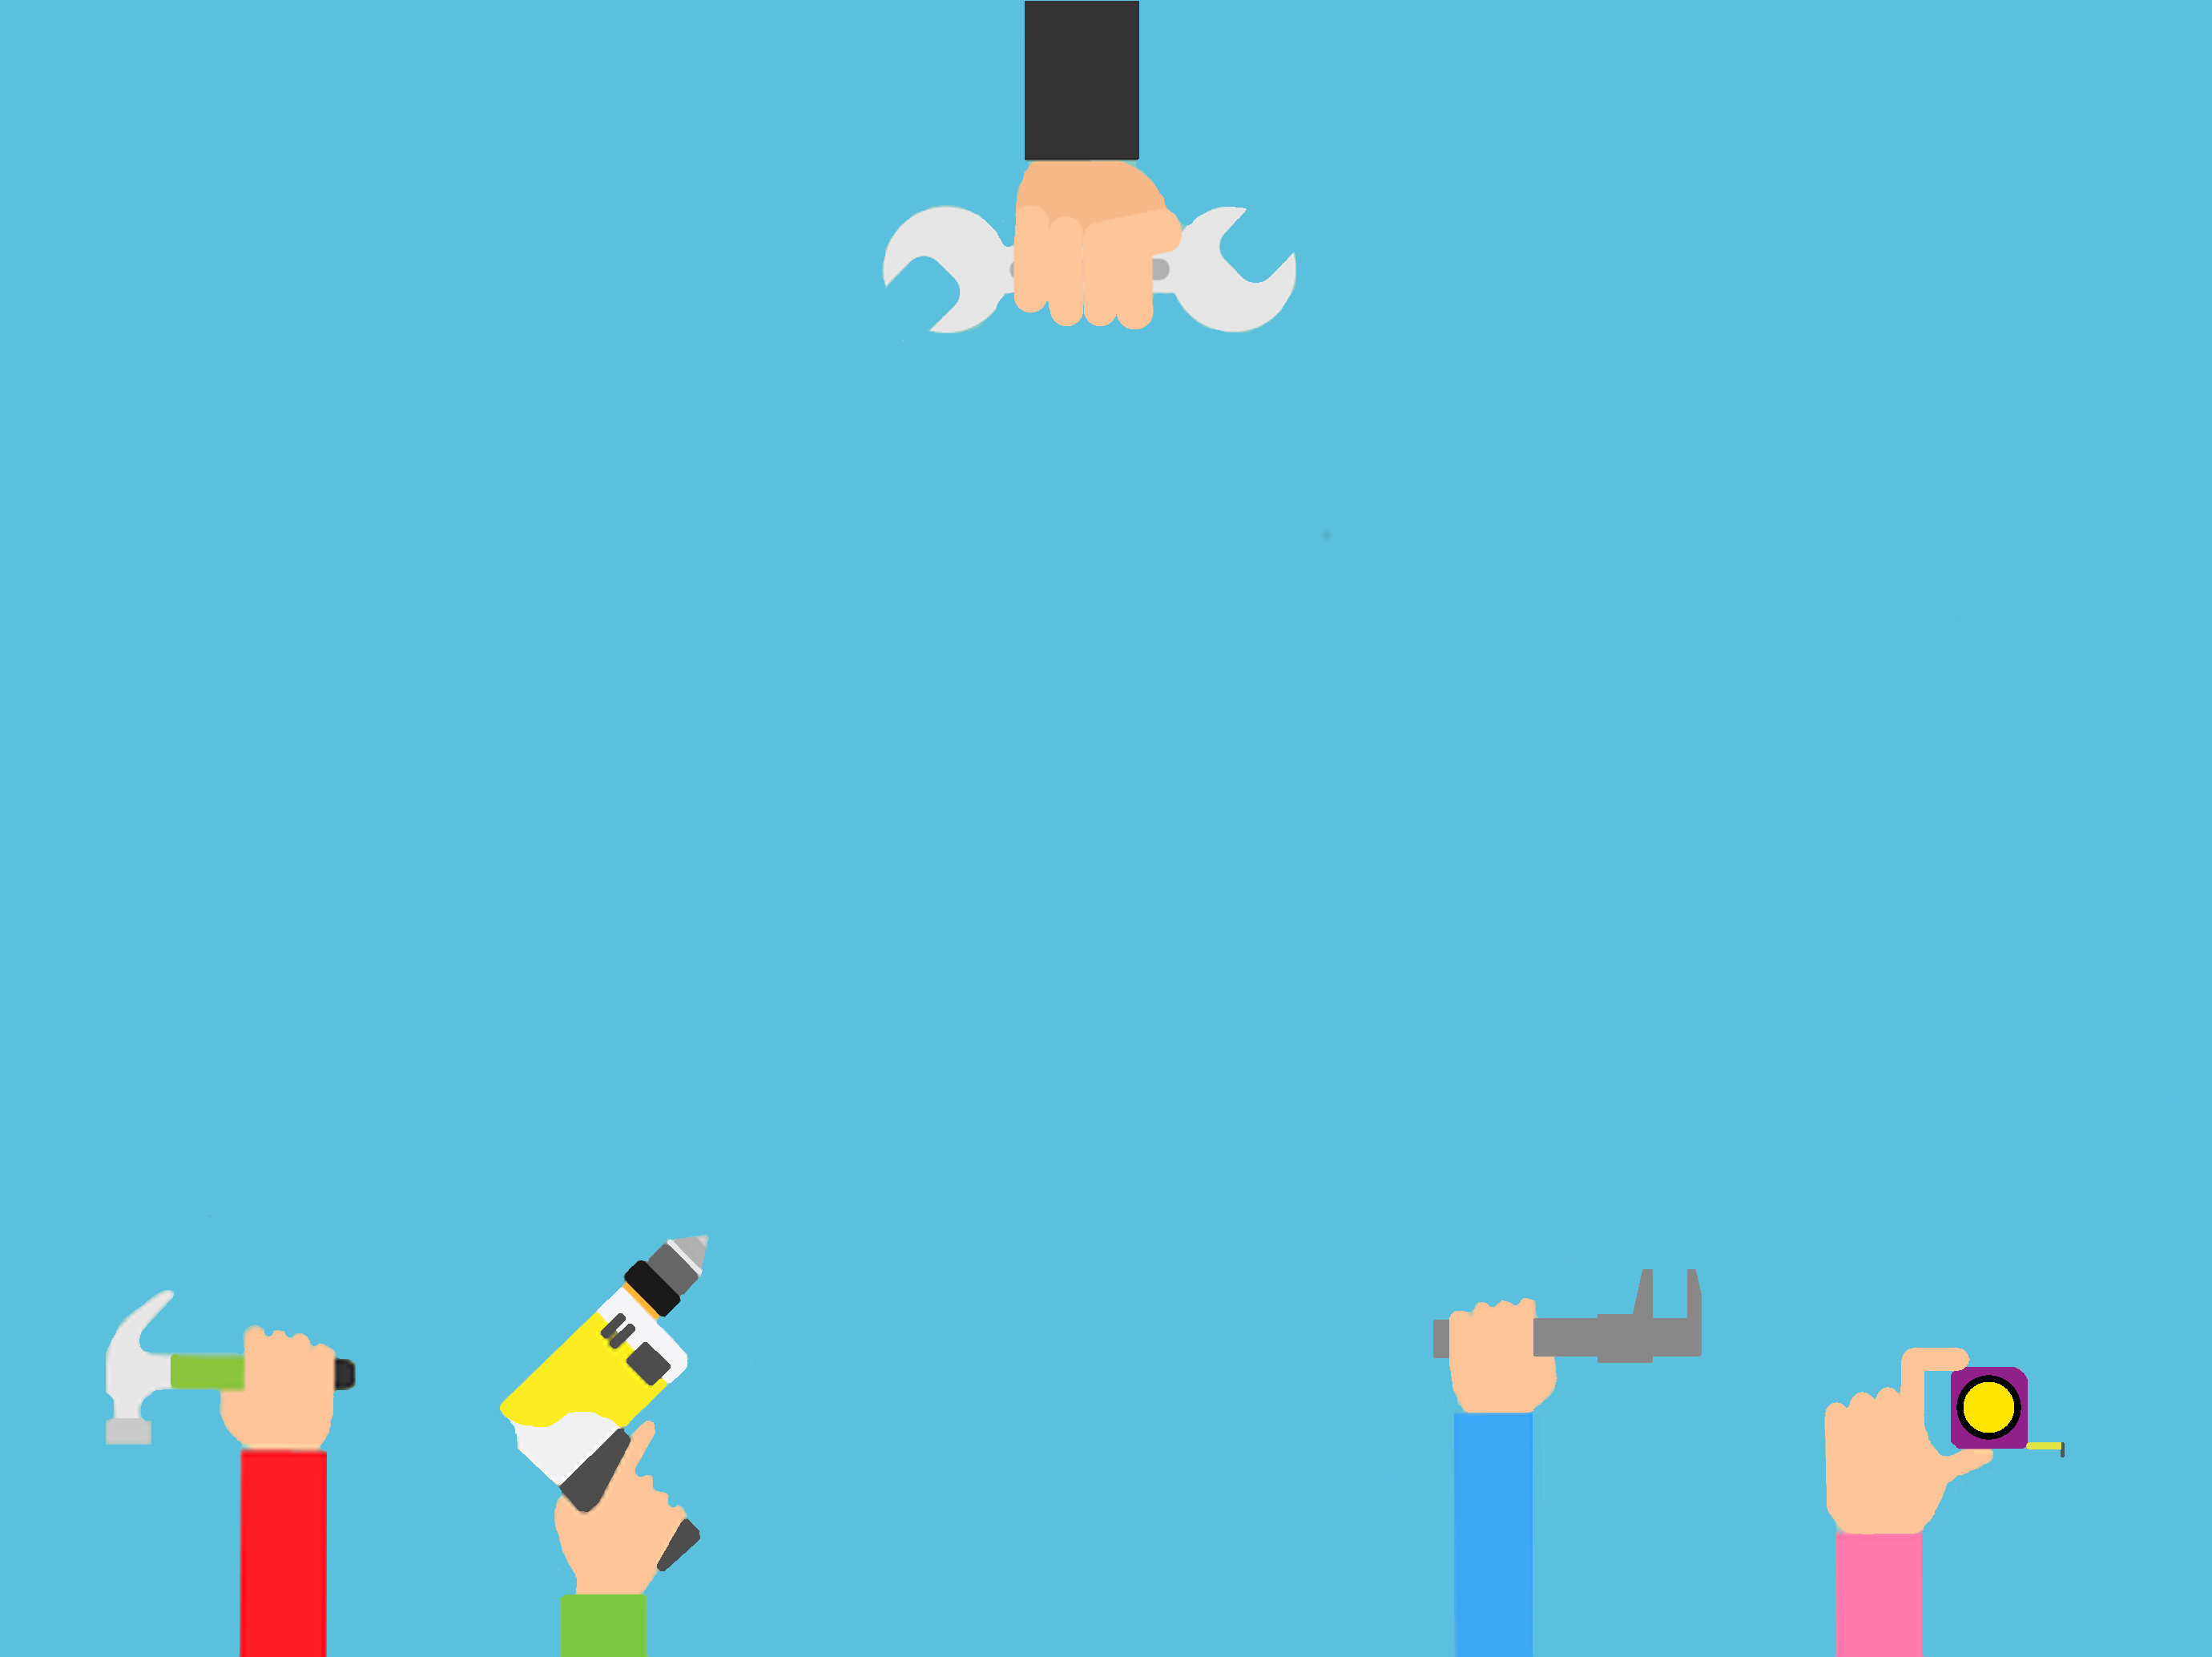
\includegraphics[width=\paperwidth]{../../img/fond}}
\frame{\titlepage}
}



\section{Introduction}

{\frame{
\frametitle{Introduction}

\begin{savoir}
Vous êtes capables :
\begin{itemize}
 \item donner certaines caractéristiques d'un matériau.
\end{itemize}
\end{savoir}

\begin{prob}
Vous devez êtes capables de choisir un procédé de fabrication en fonction:
\begin{itemize}
 \item de la géométrie d'une pièce,
 \item de son matériau,
 \item de la production associée à la pièce.
\end{itemize}
\end{prob}
}}

{\frame{
\frametitle{Propriétés et définitions}

\begin{defi}
Le soudage regroupe les procédés de jonction tendant à réaliser la continuité de l'état de matière, sous l'effet de la température ou de la pression.
\end{defi}

\begin{rem}
\begin{itemize}
 \item \textbf{Utilisation}: En raison de son faible coût, la soudure est l'un des moyens le plus utilisé dans l'assemblage de barres, de tubes, de profilés, de cornières, de plats, de tôles épaisses ou fines.
 \item \textbf{Matériaux}: Les aciers habituellement utilisés en construction sont facilement soudable.
\end{itemize}
\end{rem}
}}


{\frame{
\frametitle{Généralités}
Procédé d'assemblage permanent par fusion localisée du matériau.

\begin{itemize}
 \item \textbf{Le métal de base} :	Le métal de base constitue les pièces à assembler, de même nature ou de nature différente,
 \item \textbf{Le métal d'apport} : Le métal d'apport sert à unir les deux pièces à souder. Il intervient partiellement (en plus de la fusion du métal de base) des deux pièces à unir ou totalement (quand les deux métaux de base sont différents) dans l'élaboration du joint soudé.
 \begin{itemize}
 \item La soudure est Autogène quand le métal qui compose le joint est de même composition chimique que les pièces à souder,
 \item La soudure est Hétérogène quand le métal qui compose le joint est de nature différente des pièces à souder
 \end{itemize}
 \item \textbf{Le métal du joint} : Le métal du joint comprend le métal déposé et les bords fondus dilués. Au-delà du joint, une zone plus ou moins étendue (dite ZAT), zone thermiquement affectée, peut subir des modifications de structure
\end{itemize}
}}

\section{Procédés de soudage}

{\frame{
\frametitle{Procédés de soudage}

\begin{minipage}{0.45\linewidth}
\textbf{Électrique}
 \begin{itemize}
 	\item Arc,
 	\begin{itemize}
 	\item soudage manuel avec électrodes enrobées,
	\item soudage sous protection gazeuse:
	 \begin{itemize}
 	 \item  Avec électrode réfractaire TIG,
 	 \item  Avec électrode fusible MIG et MAG.
	 \end{itemize}
	\item soudage sous flux solide,
	\item soudage par plasma d'arc.
 	\end{itemize}
	\item Résistance.
	 \begin{itemize}
 	 \item soudage par points,
 	 \item soudage à la molette,
 	 \item soudage par bossages,
	 \item soudage en bout par étincelage,
	 \item soudage par induction.
	 \end{itemize}
	\end{itemize}
\end{minipage}\hfill
\begin{minipage}{0.45\linewidth}
\textbf{Thermochimique},
\begin{itemize}
	\item soudage aluminothermique,
	\item soudage oxyacétylénique.
\end{itemize}
 
\textbf{Mécanique}
\begin{itemize}
	\item soudage par friction, friction modelage,
	\item soudage par explosion,
	\item soudage par ultrasons,
 	\item soudage par diffusion.
 \end{itemize}
 
\textbf{Focalisé}
 \begin{itemize}
	 \item soudage par bombardement électronique,
	 \item soudage par laser.
 \end{itemize}
\end{minipage}
}}

{\frame{
\frametitle{Procédés de soudage électrique à l'arc}

\textbf{Procédé de soudage autogène par fusion}. La chaleur est produite par l'arc électrique, formé entre le métal de base et l'électrode, ou entre deux ou plusieurs électrodes.

\begin{minipage}{0.45\linewidth}

La réalisation de l'arc est conditionnée par :
\begin{itemize}
 \item la tension aux bornes de l'arc,
 \item l'intensité du courant qui le parcourt,
 \item la distance séparant les extrémités des électrodes.
\end{itemize}

L'électrode apporte le métal d'apport.
\end{minipage}\hfill
\begin{minipage}{0.5\linewidth}
 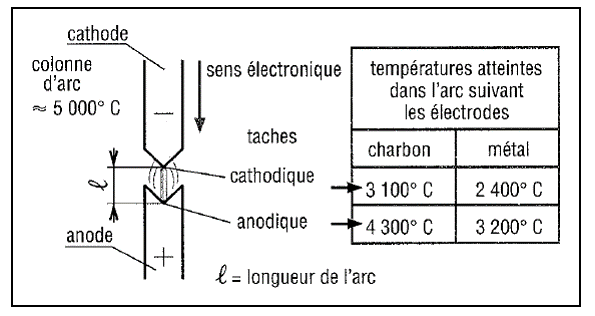
\includegraphics[width=0.9\linewidth]{img/Picture4} 
\end{minipage}
}}

{\frame{
\frametitle{Procédés de soudage électrique à l'arc}

\begin{itemize}
 \item Avantage : la fusion, très localisée, amène moins de déformation que le chalumeau et une plus grande productivité. Il est très utilisé dans l'industrie.
 \item Inconvénient majeur : le refroidissement rapide, génère de contraintes internes et des déformations parfois difficiles à corriger.
\end{itemize}

La création d'une atmosphère autour du bain de fusion :
\begin{itemize}
 \item Un gaz protège la zone du bain de fusion contre l'oxygène et l'azote de l'air,
 \item L'enrobage en fondant crée une atmosphère protégeant le bain de fusion contre l'oxygène et l'azote de l'air. Il forme également un laitier enrobant chaque goutte de métal fondu transféré de l'extrémité de l'âme jusqu'au bain de fusion.
\end{itemize}
}}	

{\frame{
\frametitle{Les techniques de soudage électrique à l'arc}

\begin{minipage}{0.6\linewidth}
\textbf{Soudage à l'électrode enrobée}\\
L'électrode, dirigée manuellement est fusible et fournit le métal d'apport. L'enrobage assure un rôle protecteur et son épaisseur permet de jouer sur la forme du cordon, concave ou convexe.
\end{minipage}\hfill
\begin{minipage}{0.35\linewidth}
 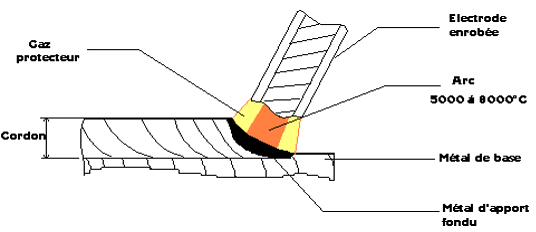
\includegraphics[width=0.95\linewidth]{img/Picture5}
\end{minipage}


\textbf{Soudage MIG (Metal Inert Gas)}\\
L'électrode fusible travaille en atmosphère inerte ( gaz protecteur : argon, argon + hélium) afin de protéger le bain de fusion. Encore appelé semi-auto, il est très adapté à la petite industrie: facile d'emploi, arc visible, pas de laitier, grande vitesse de soudage, temps de formation réduit.

\begin{minipage}{0.6\linewidth}
\textbf{Soudage MAG (Metal Active Gas)}\\
Cette variante du MIG utilise un mélange de gaz actif (gaz carbonique CO2 et d'argon), elle est adaptée aux aciers de construction au carbone.

\end{minipage}\hfill
\begin{minipage}{0.35\linewidth}
 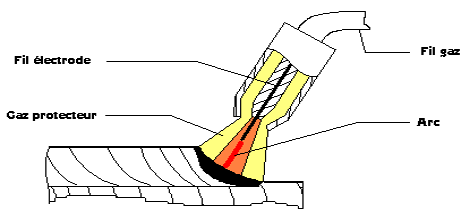
\includegraphics[width=0.95\linewidth]{img/Picture6} 
\end{minipage}
}}

{\frame{
\frametitle{Les techniques de soudage électrique à l'arc}

\textbf{Soudage TIG (Tungsten Inert Gas)}\\
Variante des précédents, plus productive et utilisant une électrode réfractaire ou non fusible en tungstène. Le métal d'apport est amené manuellement (baguette) ou automatiquement (fil déroulé) le bain de fusion et les zones avoisinantes sont protégées contre l'action de l'oxygène et de l'azote de l'air par une atmosphère de gaz neutre dit inerte, généralement de l'argon.

\begin{minipage}{0.35\linewidth}
 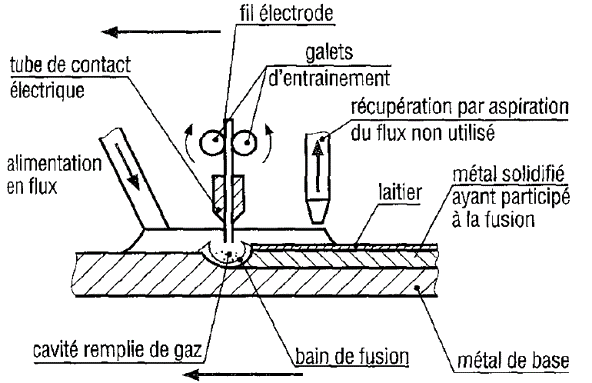
\includegraphics[width=0.95\linewidth]{img/Picture7}
\end{minipage}\hfill
\begin{minipage}{0.6\linewidth}
\textbf{Soudage électrique à l'arc sous flux solide}
Ce procédé consiste à effectuer un joint de soudure sur de l'acier à l'aide d'un arc électrique qui est submergé de flux en poudre.
\end{minipage}

\vspace{-0.5cm}

\begin{minipage}{0.6\linewidth}
\textbf{Soudage électrique à l'arc au plasma}
Le soudage au plasma est en fait un soudage T.I.G. dans lequel l'arc est étranglé (ou confiné) dans une tuyère.
\end{minipage}\hfill
\begin{minipage}{0.35\linewidth}
 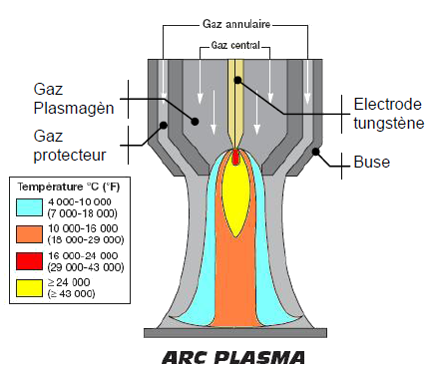
\includegraphics[width=0.8\linewidth]{img/Picture8} 
\end{minipage}
}}

{\frame{
\frametitle{Les techniques de soudage électrique à résistance}

\begin{minipage}{0.6\linewidth}
\textbf{Procédé de soudage électrique par points}\\
La soudure est réalisé entre deux électrodes. Les pièces à assembler sont maintenues en contact par un effort de compression puis soudées par recouvrement ou bout à bout sans métal d'apport.
\end{minipage}\hfill
\begin{minipage}{0.35\linewidth}
 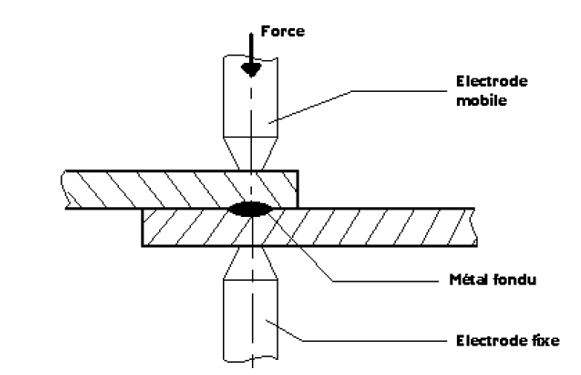
\includegraphics[width=0.95\linewidth]{img/Picture9}
\end{minipage}

\begin{minipage}{0.6\linewidth}
\textbf{Procédé de soudage électrique à la molette}\\
Les électrodes sont remplacées par des molettes tournantes ce qui permet un soudage continu ou discontinu très rapide.
\end{minipage}\hfill
\begin{minipage}{0.35\linewidth}
 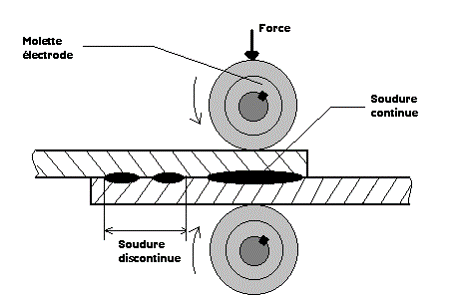
\includegraphics[width=0.95\linewidth]{img/Picture10} 
\end{minipage}

\textbf{Procédé de soudage électrique par bossages}\\
Autre variante, ce procédé permet de souder plusieurs points en même temps. Les électrodes sont remplacées par des plateaux permettant de souder des formes et treillis, des tubes superposés et croisés.

}}

{\frame{
\frametitle{Les techniques de soudage électrique à résistance}

\textbf{Procédé de soudage électrique en bout par étincelage}\\
Les pièces à souder sont maintenues par des mâchoires, et sont mises en contact puis chauffées par effet Joule (petites sections), soit par étincelage (fortes sections). Après coupure du courant, un refoulement "forge" la soudure.

\textbf{Soudage par impulsion magnétique}\\
Un champ magnétique circule dans l'anneau ce qui provoque un courant induit dans les deux pièces qui montent alors en température. Au moment de la fusion du métal un important effort axial permet l'assemblage.

\begin{center}
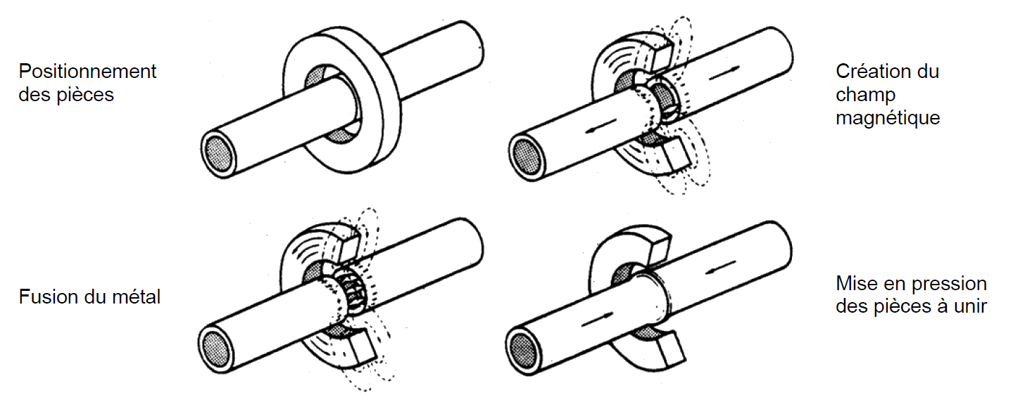
\includegraphics[width=0.7\linewidth]{img/Picture11}
\end{center}

}}

{\frame{
\frametitle{Les techniques de soudage mécanique}

\textbf{Procédé de soudage mécanique par friction}\\
Un échauffement est crée entre deux pièces pressées et en mouvement l'une par rapport à l'autre.

\begin{center}
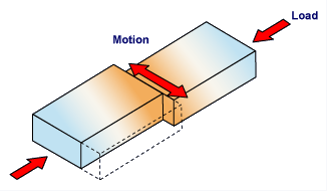
\includegraphics[width=0.35\linewidth]{img/Picture12}\hfill
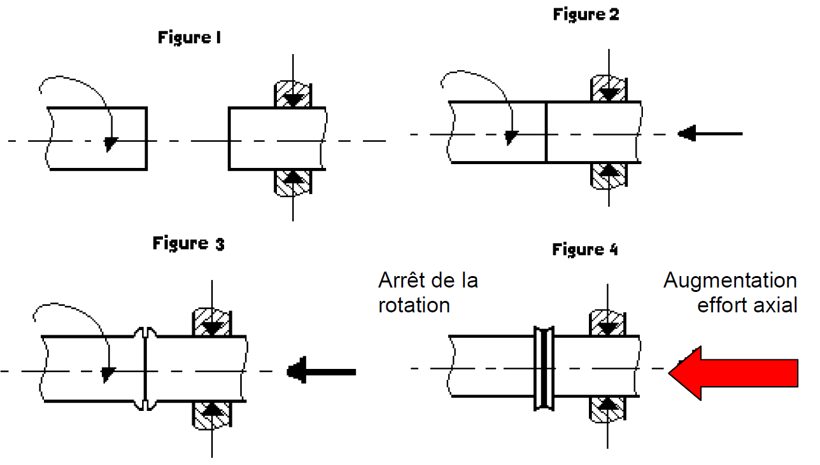
\includegraphics[width=0.57\linewidth]{img/Picture13}
\end{center}
}}

{\frame{
\frametitle{Les techniques de soudage mécanique}

\begin{minipage}{0.6\linewidth}
\textbf{Procédé de soudage par explosion}\\
Essentiellement employée pour assembler des métaux de nature différente (ex: superstructures en aluminium sur un bateau à coque en acier pour abaisser le centre de gravité). Les métaux à assembler sont superposés selon un certain angle et recouverts d'une couche uniforme d'explosif, la combustion provoque la fusion.
\end{minipage}\hfill
\begin{minipage}{0.35\linewidth}
 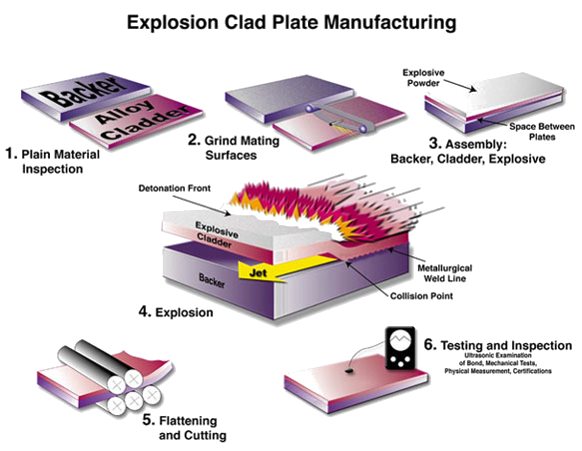
\includegraphics[width=0.8\linewidth]{img/Picture14} 
\end{minipage}

\begin{minipage}{0.7\linewidth}
\textbf{Procédé de soudage par ultrason}\\
Des vibrations de haute fréquence 20, 30, 35, 40 et 70 kHz sont envoyées aux deux pièces par le biais d'un outil vibrant appelé sonotrode ou tête de soudure. Les amplitudes des vibration varient entre 10 et 120 micromètres, La soudure se fait grâce à la chaleur engendrée à l'interface des deux pièces.
\end{minipage}\hfill
\begin{minipage}{0.25\linewidth}
 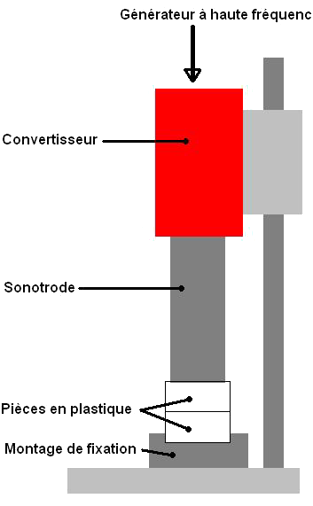
\includegraphics[width=0.7\linewidth]{img/Picture15} 
\end{minipage}
}}

{\frame{
\frametitle{Les techniques de soudage focalisé}

\begin{minipage}{0.7\linewidth}
\textbf{Procédé de soudage par bombardement électronique}\\
Réalise un soudage autogène sous vide, généralement sans métal d'apport, en utilisant un faisceau d'électrons.
\end{minipage}\hfill
\begin{minipage}{0.25\linewidth}
 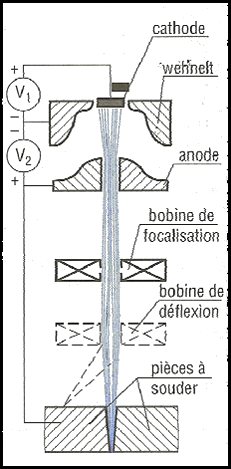
\includegraphics[width=0.65\linewidth]{img/Picture16} 
\end{minipage}

\begin{minipage}{0.7\linewidth}
\textbf{Procédé de soudage au laser}\\
Le faisceau laser est une source de chaleur extrêmement concentrée qui permet des soudages étroits, profonds, à une cadence rapide.
\end{minipage}\hfill
\begin{minipage}{0.25\linewidth}
 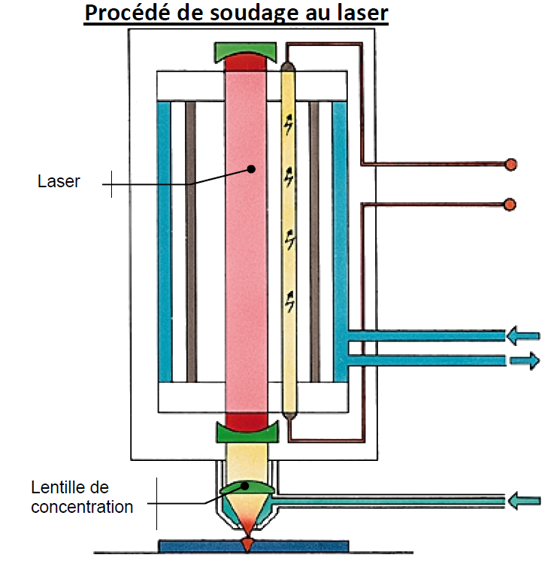
\includegraphics[width=0.85\linewidth]{img/Picture17} 
\end{minipage}
}}

{\frame{
\frametitle{Les techniques de soudage thermochimiques}

\begin{minipage}{0.65\linewidth}
\textbf{Procédé de soudage oxyacétylénique}
C'est un procédé de soudure par fusion où la chaleur de soudure est produite par la combustion de gaz mélange d'oxygène et d'acétylène à l'extrémité d'un chalumeau.\\
L'épaisseur des pièces à souder est inférieure à 8 mm pour les métaux lourds, et de 15 mm pour les métaux légers.
\end{minipage}\hfill
\begin{minipage}{0.3\linewidth}
 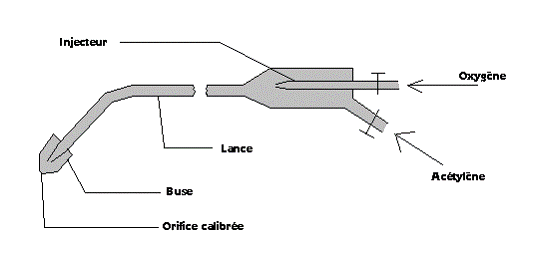
\includegraphics[width=0.9\linewidth]{img/Picture18}\\
 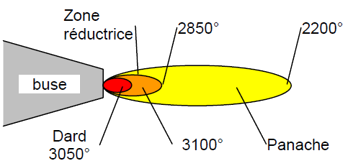
\includegraphics[width=0.9\linewidth]{img/Picture19}
\end{minipage}

~\

\begin{minipage}{0.65\linewidth}
\textbf{Procédé de soudage aluminothermique}\\
De la poudre d'allumage est placé sur une charge (appelée \og thermit \fg) dans un creuset métallique. La réaction du mélange composé d'aluminium granulé (0,5 à 2 mm) et d'oxyde de fer pulvérulent provoque une brusque élévation de température qui fond le métal. Cela permet le soudage sur place de grosses pièces en acier (rails de chemin de fer)
\end{minipage}\hfill
\begin{minipage}{0.3\linewidth}
 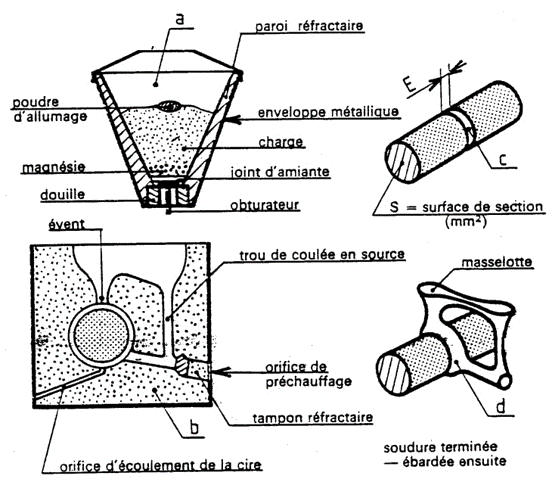
\includegraphics[width=0.95\linewidth]{img/Picture20} 
\end{minipage}
}}








{\frame{
\frametitle{Autre procédés d'assemblage non démontable}

\begin{minipage}{0.7\linewidth}
\textbf{Le brasage}
\begin{itemize}
 \item La brasure est un assemblage toujours hétérogène. Les pièces à assembler (métal de base) sont chauffées en présence d'un métal ou alliage différent (métal d'apport),
 \item La température de fusion du métal d'apport est inférieure à celle du métal de base,
 \item La formation du joint ou cordon est assurée par la seule intervention du métal d'apport qui agit comme une \og colle \fg.
\end{itemize}

~\

\textbf{Le soudobrasage}\\
Le soudobrasage est différent du brasage car les pièces à assembler ne sont en général pas chauffées.
\end{minipage}\hfill
\begin{minipage}{0.25\linewidth}
 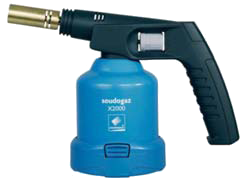
\includegraphics[width=0.9\linewidth]{img/Picture2} \\ \vfill
 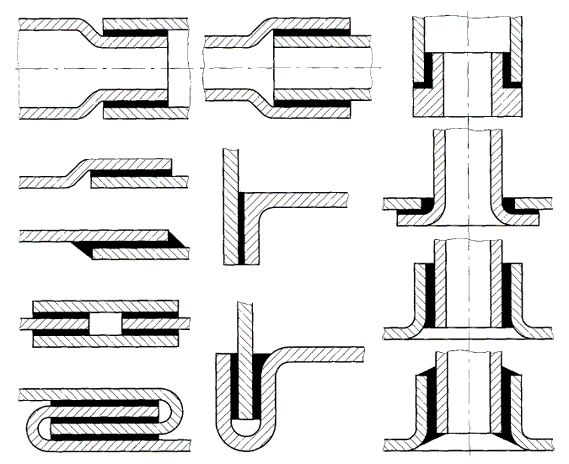
\includegraphics[width=0.9\linewidth]{img/Picture3} 
\end{minipage}
}}

{\frame{
\frametitle{Comparaison économique des procédés}

\begin{center}
 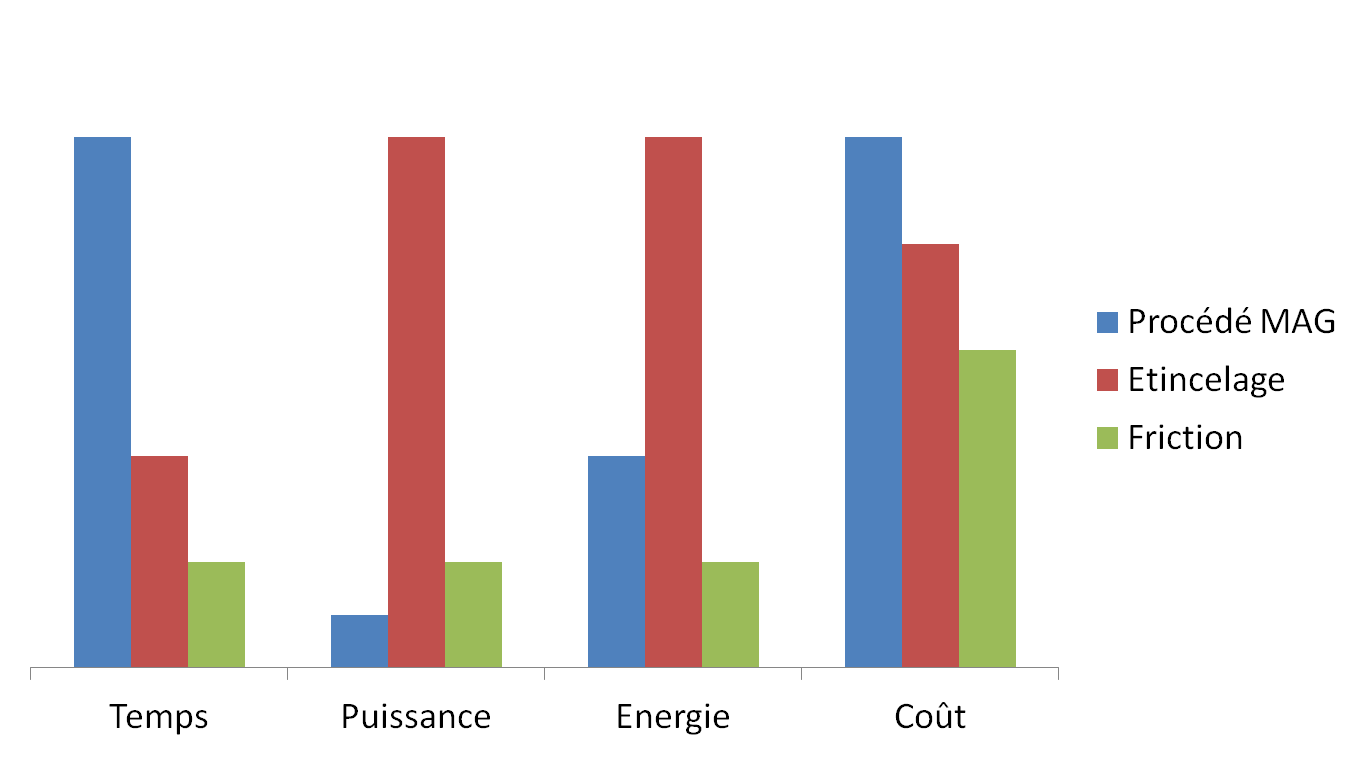
\includegraphics[width=0.85\linewidth]{img/Picture21} 
\end{center}
}}

{\frame{
\frametitle{Avantages de la soudure}

\textbf{Procédés concurrents}
\begin{itemize}
 \item Les assemblages mécaniques (boulonnage, vissage, rivetage, sertissage, clinchage,...) n'assurent pas une continuité du métal, et ne conviennent pas à toutes les gammes d'épaisseur des métaux,
 \item Les assemblages par collage seulement pour les produits minces, faiblement sollicités, et ont une durabilité réduite.
\end{itemize}

\textbf{Avantages du soudage}
\begin{itemize}
 \item Continuité de la pièce qui confère ainsi à l'assemblage des caractéristiques équivalentes à celles du matériau de base (mécaniques, thermiques, chimiques, électriques, d'étanchéité, de durabilité,...),
 \item Il peut donc, selon le procédé, assurer l'étanchéité de la pièce soudée.
Rapide et économique il est aussi durable, car insensible aux variations de température et aux conditions climatiques
\end{itemize}
}}

{\frame{
\frametitle{Défauts de la soudure}

\begin{itemize}
 \item \textbf{Fragilité produite par la ségrégation}: Le chauffage local du métal produit un traitement thermique local. Il y a donc une modification locale de la microstructure et de l'état métallurgique de la zone du métal affectée par le chauffage (ZAT : zone affectée thermiquement),
 \item \textbf{Corrosion au cordon de soudure}: La juxtaposition de métaux différents peut avoir un phénomène de corrosion galvanique,
 \item \textbf{Porosités}: Il s'agit de défauts sphériques creux qui peuvent être ou non débouchants,
 \item \textbf{Soufflures}: Ce terme désigne un groupe de porosités non débouchants,
 \item \textbf{Inclusions}: Elles désignent un composé étranger à la soudure,
 \item \textbf{Retassures}: Suite à un retrait du métal lors de son refroidissement, l'espace vide formé apparaît visuellement à la surface du cordon, ainsi qu'à l'intérieur du cordon,
 \item \textbf{Criques de solidification}: Défauts semblables aux retassures mais non apparents.
\end{itemize}
}}

{\frame{
\frametitle{Défauts de la soudure}

\begin{itemize}
 \item \textbf{Excès de pénétration}: Métal débordant du côté envers du cordon,
 \item \textbf{Collage ou manque de pénétration}: Le métal de base n'est pas fondu, ce qui diminue la section efficace de la soudure,
 \item \textbf{Morsures}: Défaut où le métal de base est \og creusé \fg sur une partie du cordon,
 \item \textbf{Fissures}: La fissuration à froid est causée par des contraintes mécaniques résiduelles importantes,
 \item \textbf{Caniveaux}: Morsure de grande taille proportionnellement à la grandeur du métal de base due à une trop grande chaleur du métal d'apport par rapport à l'épaisseur,
 \item \textbf{Pollution ferreuse}: Corrosion des aciers inoxydables causée par la destruction de la couche de passivation et activée par la présence de fer,
 \item \textbf{Défauts géométriques}: Peuvent être des défauts d'alignement entre les pièces, un cordon trop bombé...
\end{itemize}
}}

{\frame{
\frametitle{Principaux matériaux soudables}

L'aptitude au soudage est qualifiée par le degrés de soudabilité du matériau.

\textbf{Soudage des aciers}
 \begin{itemize}
  \item La soudabilité d'un acier dépendra de son pourcentage de carbone. Un pourcentage de carbone élevé rends difficile le soudage,
   \begin{itemize}
    \item La majorité des aciers de constructions, type S ou E, sont soudables parce que faiblement alliés et pauvres en carbones ($\%C<0,5$),
    \item Les aciers inoxydables à condition que le pourcentage de carbone ($\%C$) reste inférieur à $0,05\%$,
    \item Les aciers de type C et les aciers faiblement alliés, ont un titrage en carbone qui favorise la trempe.
   \end{itemize}
  \item La soudabilité peut être estimée par le calcul du pourcentage de carbone équivalent ($C_{eq}$) exprimé en pourcentage de masse.
	$C_{eq}=\%C+ (\%Cr+\%Mo+\%V) /5+\%Mn /6+ (\%Ni+\%Cu)/15$
	\begin{itemize}
	 \item Si $C_{eq}< 0,4$ : l'acier est parfaitement soudable à température ambiante,
	 \item Si $0,45 < C_{eq} < 0,7$ : l'acier est moyennement soudable, préchauffage de 100 à 400°C,
	 \item Si $C_{eq} > 0,7$ : l'acier est difficilement soudable, préchauffage, électrodes spéciales, traitements thermiques..
\end{itemize}
\end{itemize}
}}

{\frame{
\frametitle{Principaux matériaux soudables}

\textbf{Les fontes}\\
Leur soudage est en général très difficile (électrodes spéciales, préchauffage,?) et donc utilisé en réparation ou en rechargement de pièces accidentées ou usées.

\textbf{Les alliages d'aluminium}\\
Les alliages sans durcissement structural (aluminium pur, Al + Mg, Al + Mn, Al + Si) ont une bonne soudabilité (TIG ou MIG).\\
Les alliages à durcissement structural (Al + Mg + Si, Al + Cu, Al + Zn + Mg) sont un peu plus difficiles à souder (MIG) et nécessitent plus de précautions.

\textbf{Les matières plastiques}\\
L'assemblage des polymères se fait par des moyens spécifiques tels que les lasers à diodes ou les ultrasons.
}}

\section{Représentation des soudures}

{\frame{
\frametitle{Les formes de joints}

\begin{center}
 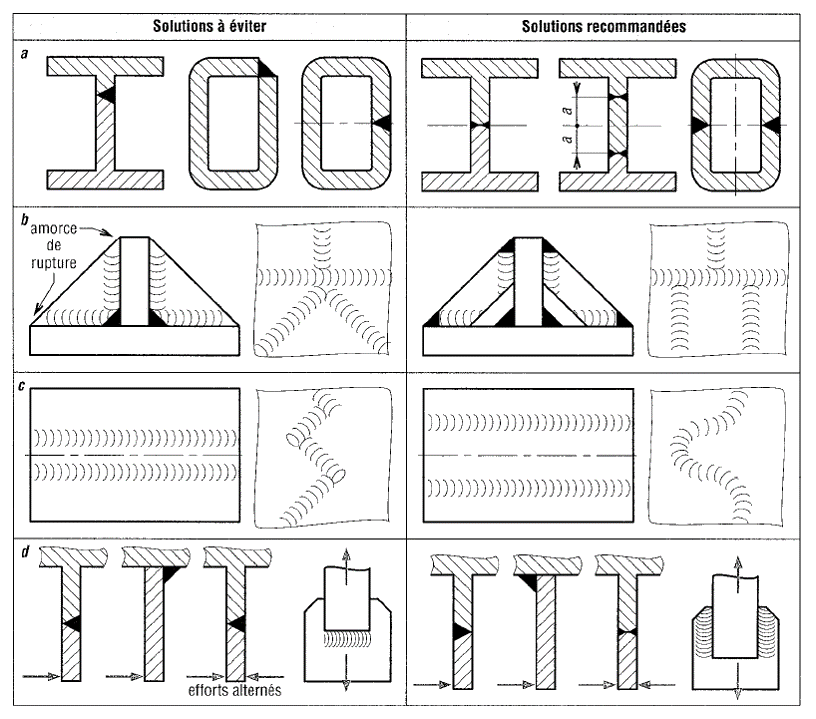
\includegraphics[width=0.7\linewidth]{img/Picture22}
\end{center}
}}

{\frame{
\frametitle{La représentation des joints}

\begin{center}
 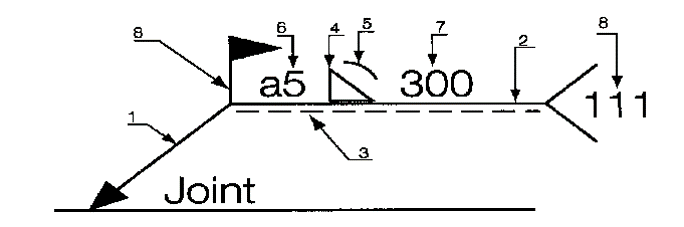
\includegraphics[width=0.8\linewidth]{img/Picture23}\\
 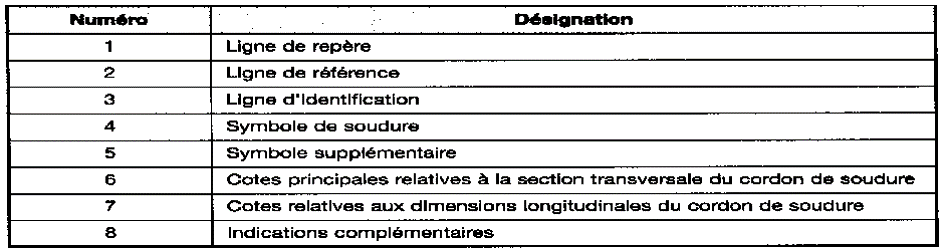
\includegraphics[width=0.8\linewidth]{img/Picture24}
\end{center}
}}

{\frame{
\frametitle{La représentation des joints}

\textbf{La ligne de repère (1)}

\begin{center}
 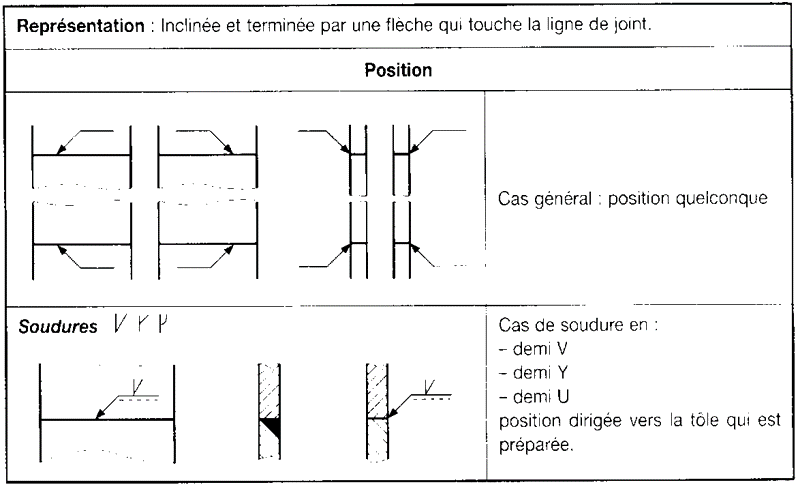
\includegraphics[width=0.6\linewidth]{img/Picture25}
\end{center}

\textbf{La ligne de référence et d'identification (2) et (3)}

Représentation: Elles doivent être tracées de préférence parallèles au bord inférieur du dessin. La ligne d'identification (trait interrompu) peut être tracée au dessus ou au dessous de la ligne de référence (trait continu).
}}

{\frame{
\frametitle{La représentation des joints}

\textbf{Le symbole de soudure (4)}

\begin{center}
 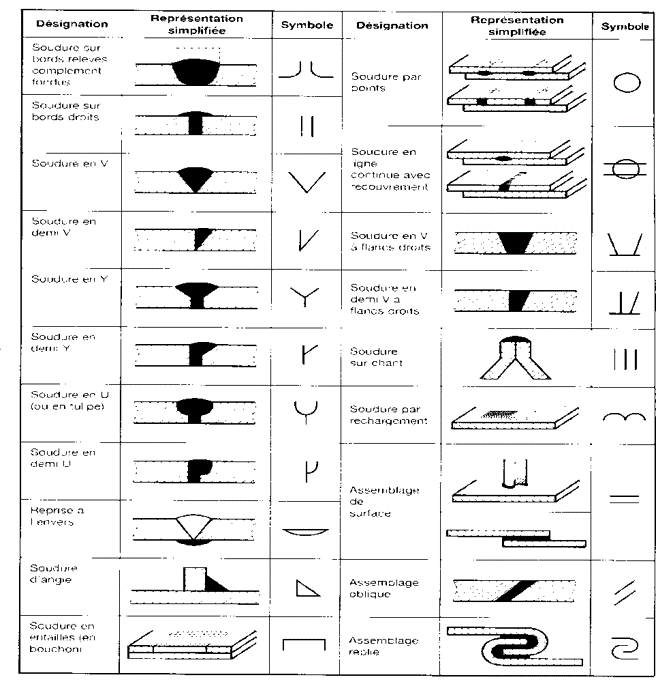
\includegraphics[width=0.55\linewidth]{img/Picture26}
\end{center}
}}

{\frame{
\frametitle{La représentation des joints}

\textbf{Le symbole supplémentaire (5)}

\begin{center}
 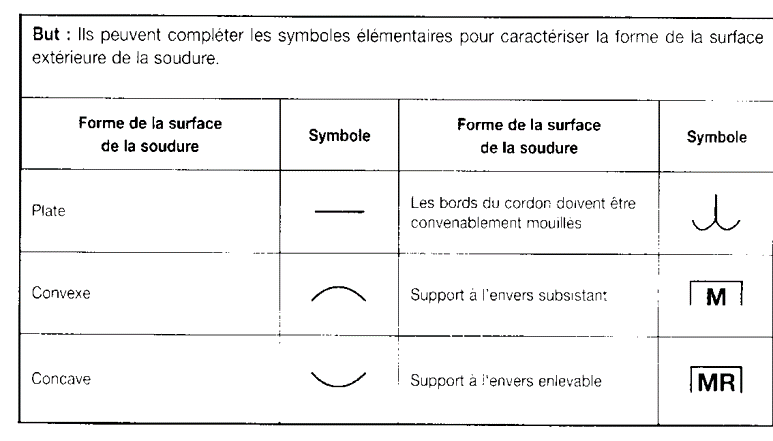
\includegraphics[width=0.8\linewidth]{img/Picture27}
\end{center}
}}

{\frame{
\frametitle{Exemples de symboles}

\begin{center}
 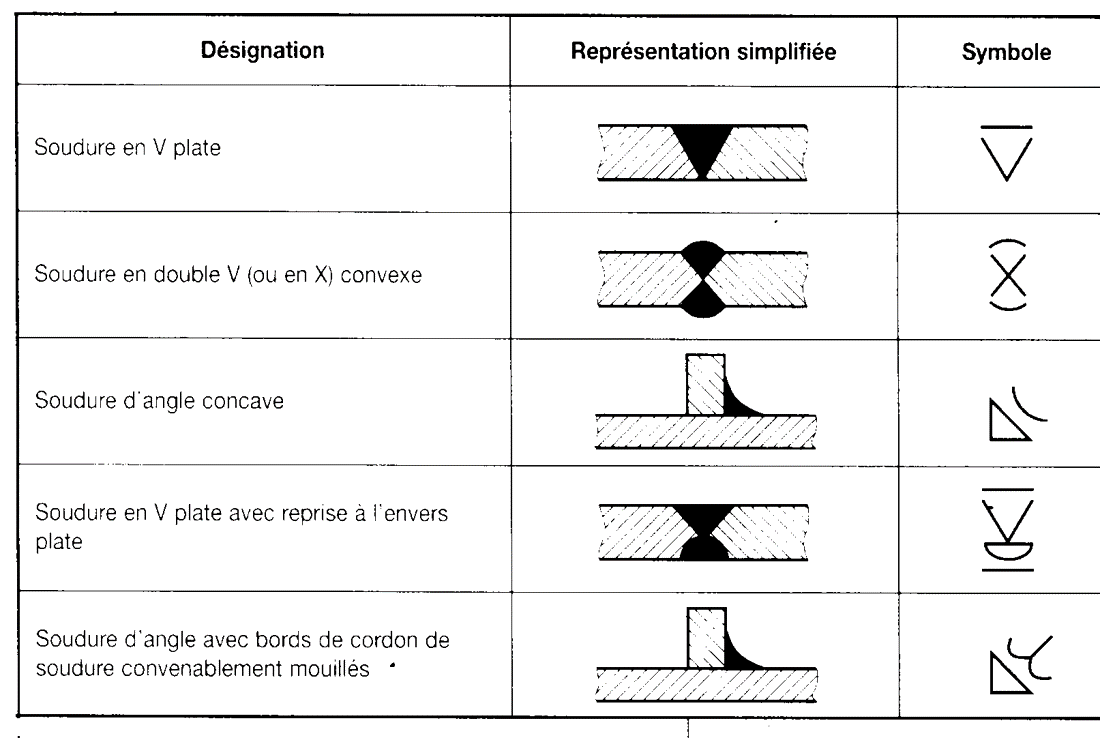
\includegraphics[width=0.8\linewidth]{img/Picture28}
\end{center}
}}

{\frame{
\frametitle{La représentation des joints}

\textbf{La cotation des soudures (6) et (7)}

\begin{center}
 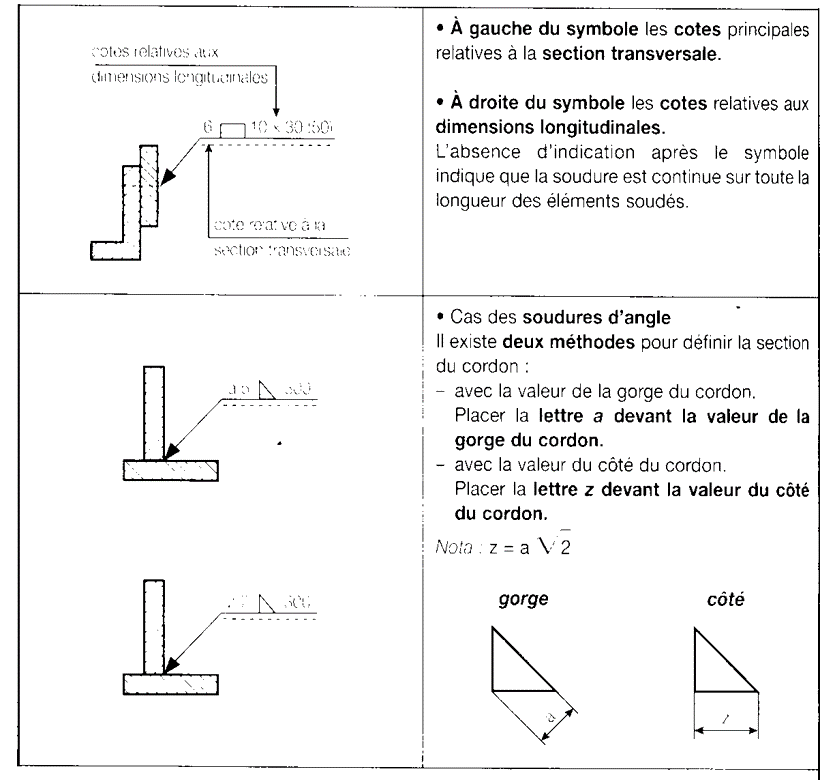
\includegraphics[width=0.5\linewidth]{img/Picture29}
\end{center}
}}

{\frame{
\frametitle{La représentation des joints}

\begin{center}
 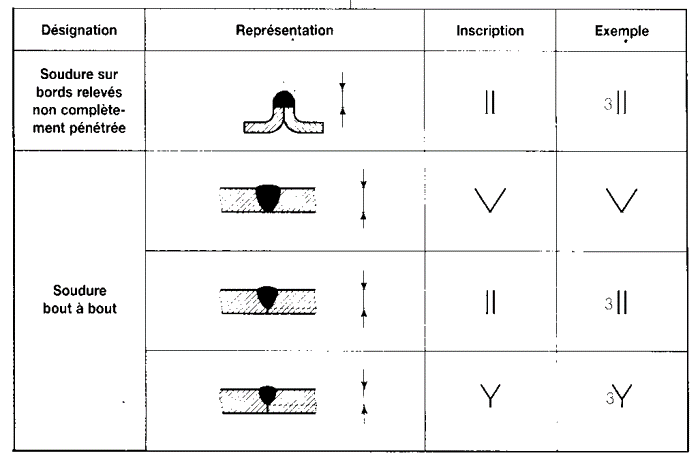
\includegraphics[width=0.8\linewidth]{img/Picture30}
\end{center}
}}

{\frame{
\frametitle{La représentation des joints}

\begin{center}
 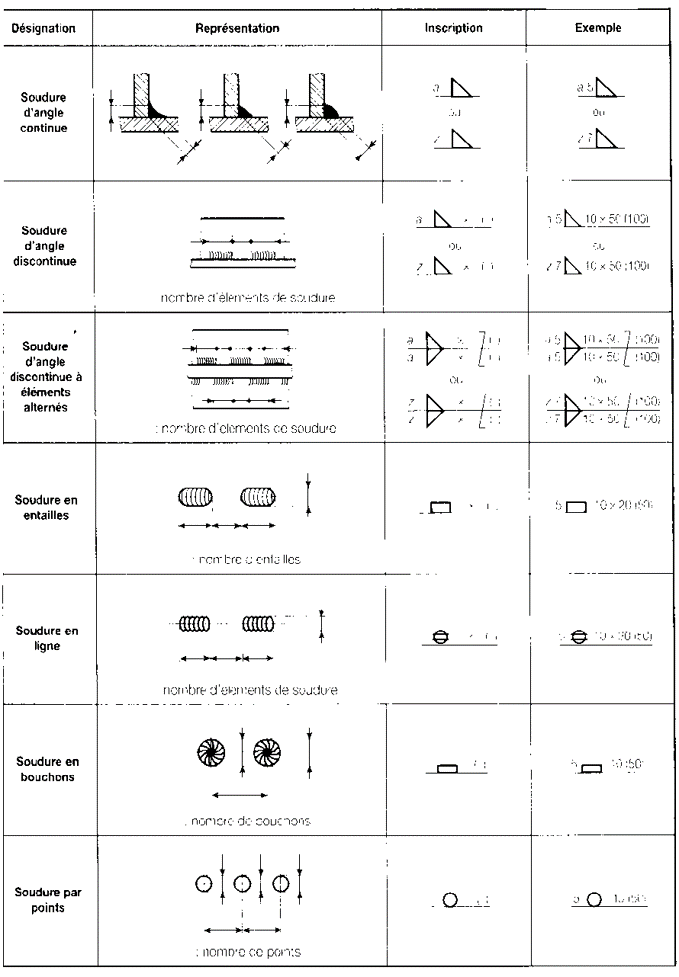
\includegraphics[angle=90,width=0.8\linewidth]{img/Picture31}
\end{center}
}}

{\frame{
\frametitle{La représentation des joints}

\begin{center}
 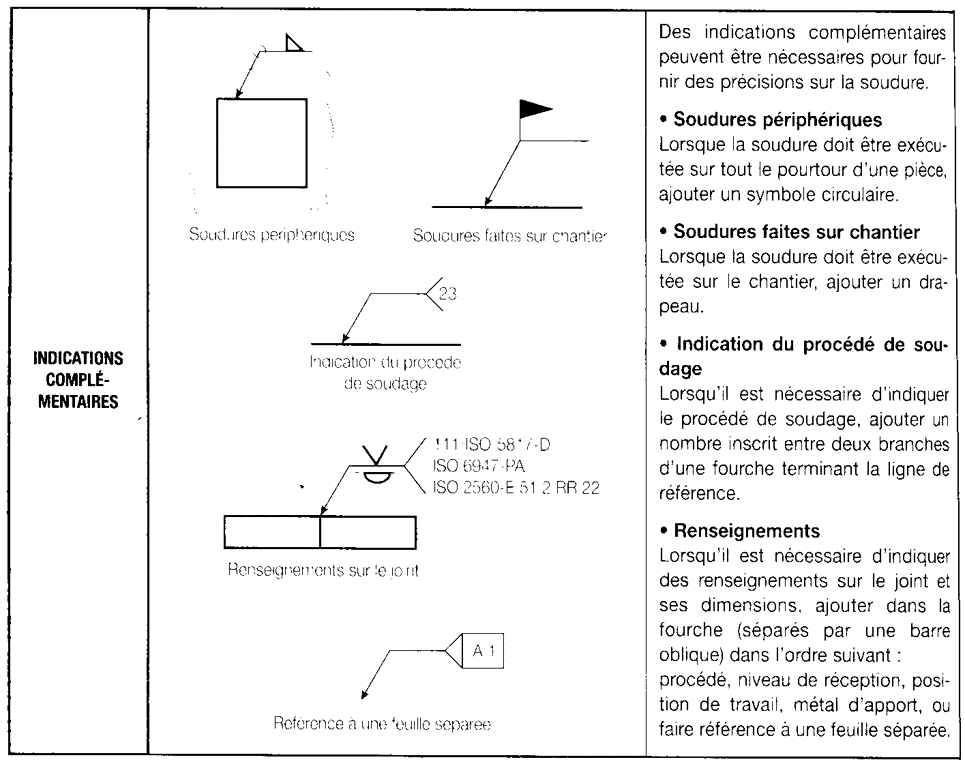
\includegraphics[width=0.8\linewidth]{img/Picture32}
\end{center}
}}

{\frame{
\frametitle{La représentation des joints}

\begin{center}
 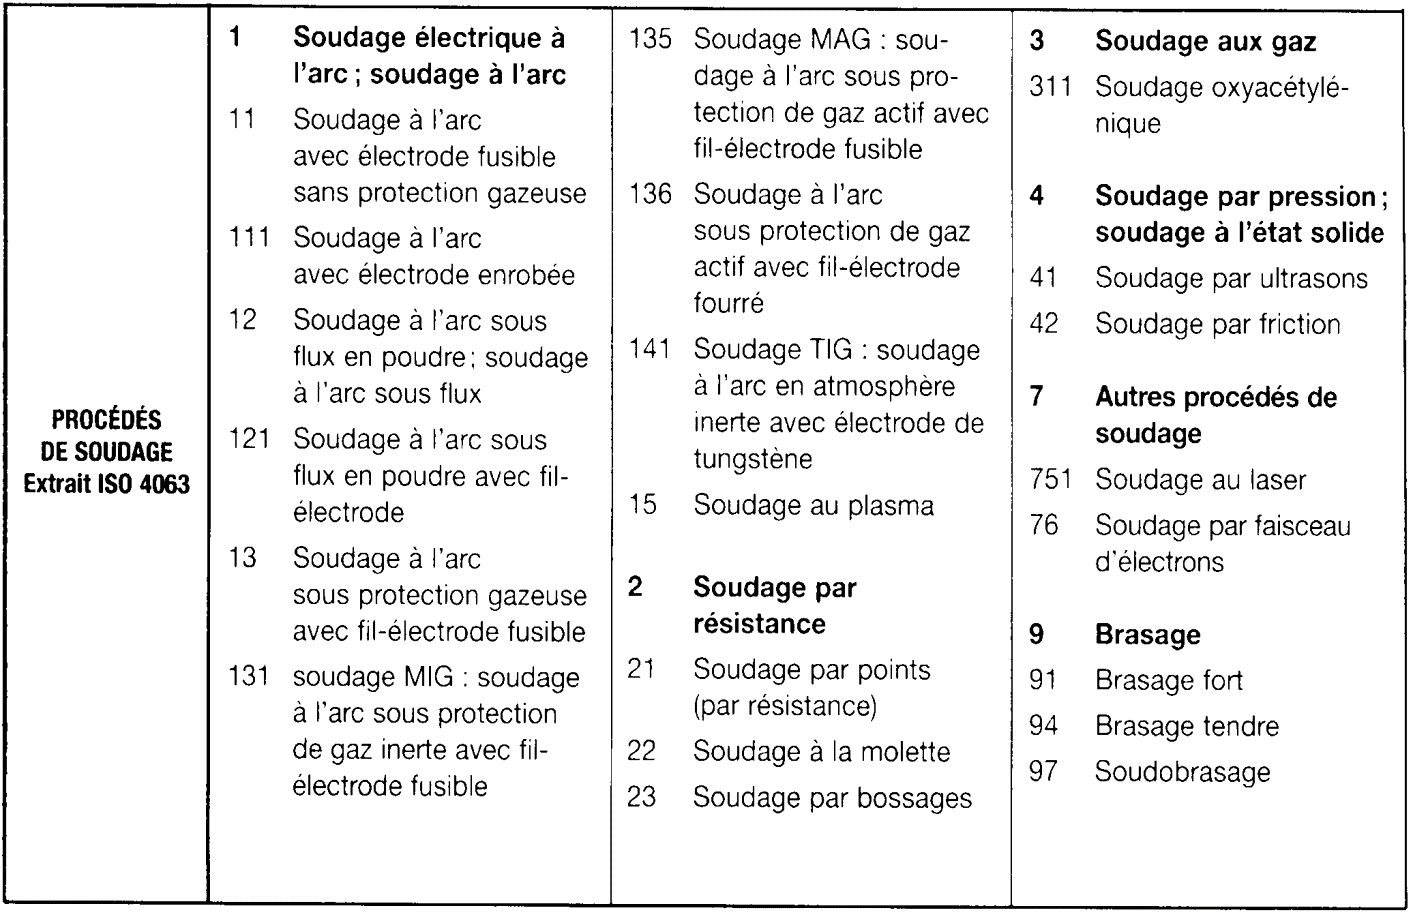
\includegraphics[width=0.8\linewidth]{img/Picture33}
\end{center}
}}

{\frame{
\frametitle{La représentation des joints}

\begin{center}
 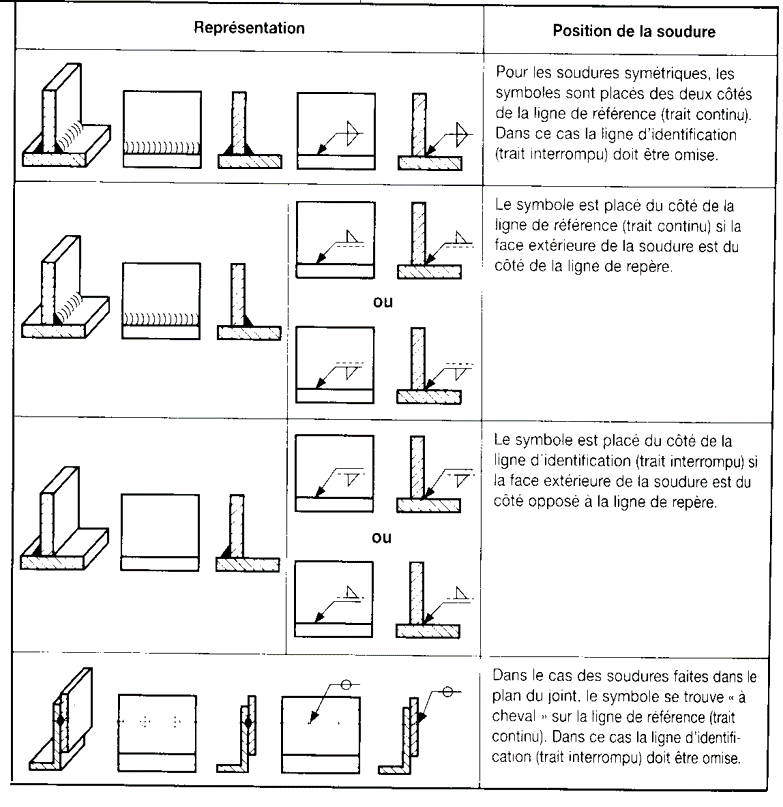
\includegraphics[width=0.6\linewidth]{img/Picture34}
\end{center}
}}

{\frame{
\frametitle{La représentation des joints}

\begin{center}
 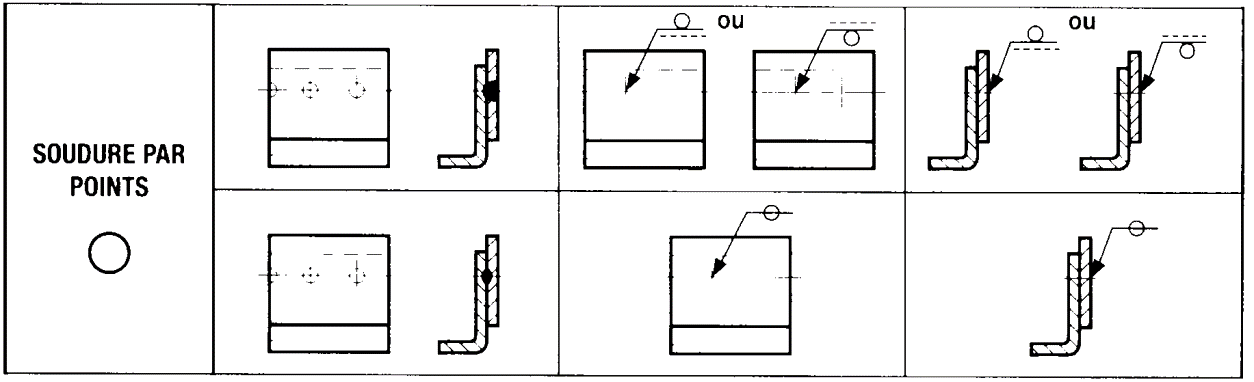
\includegraphics[width=0.8\linewidth]{img/Picture36}
\end{center}
}}

{\frame{
\frametitle{La représentation des joints}

\begin{center}
 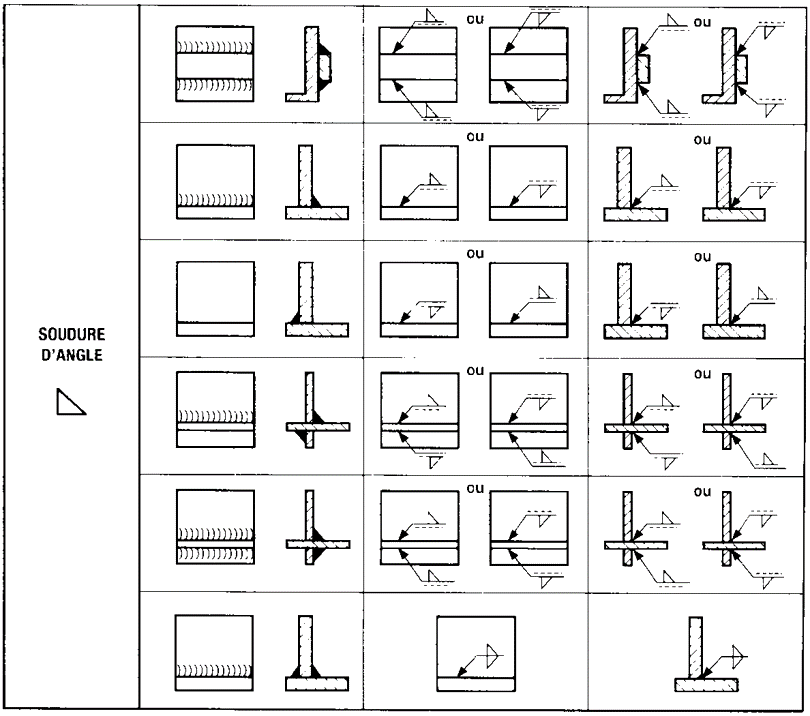
\includegraphics[width=0.7\linewidth]{img/Picture38}
\end{center}
}}

{\frame{
\frametitle{Conclusion}

\begin{savoir}
Vous êtes capables :
\begin{itemize}
 \item de concevoir une pièce mécano-soudée,
 \item de représenter des joints de soudure.
\end{itemize}
\end{savoir}

\begin{prob}
Vous devez êtes capables :
 \begin{itemize}
 \item de concevoir une pièce moulée.
 \end{itemize}
\end{prob}
}}


\end{document}